\documentclass{standalone}
\usepackage{tikz}
\usepackage{color}
\usepackage{bm}
\usepackage{amssymb}
\usepackage{tkz-euclide}
\usetikzlibrary{arrows.meta}
\usetikzlibrary{positioning}
\usetikzlibrary{calc}
\usetikzlibrary{circuits.ee.IEC}

\renewcommand{\vector}[3][cyan]{
    \begin{scope}[local bounding box=#2]
        \coordinate(anchor) at #3;
        \draw[draw=black, ultra thin, fill=#1!10] ($(anchor)$) rectangle ++(0.3,0.3);
        \draw[draw=black, ultra thin, fill=#1!30] ($(0.3,0) + (anchor)$) rectangle ++(0.3,0.3);
        \draw[draw=black, ultra thin, fill=#1!50] ($(0.6,0) + (anchor)$) rectangle ++(0.3,0.3);
    \end{scope}
}
\newcommand{\vectorDark}[3][cyan]{
    \begin{scope}[local bounding box=#2]
        \coordinate(anchor) at ($#3 + (-0.15,-0.15)$);
        \draw[draw=black, ultra thin, fill=#1!30] ($(anchor)$) rectangle ++(0.3,0.3);
        \draw[draw=black, ultra thin, fill=#1!50] ($(-0.3,0) + (anchor)$) rectangle ++(0.3,0.3);
        \draw[draw=black, ultra thin, fill=#1!70] ($(0.3,0) + (anchor)$) rectangle ++(0.3,0.3);
    \end{scope}
}
\newcommand{\vectorDarkDark}[3][cyan]{
    \begin{scope}[local bounding box=#2]
        \coordinate(anchor) at ($#3 + (-0.15,-0.15)$);
        \draw[draw=black, ultra thin, fill=#1!50] ($(anchor)$) rectangle ++(0.3,0.3);
        \draw[draw=black, ultra thin, fill=#1!70] ($(-0.3,0) + (anchor)$) rectangle ++(0.3,0.3);
        \draw[draw=black, ultra thin, fill=#1!90] ($(0.3,0) + (anchor)$) rectangle ++(0.3,0.3);
    \end{scope}
}
\newcommand{\embedding}[3][cyan]{
    \begin{scope}[local bounding box=#2]
        \coordinate(anchor) at ($#3 + (-0.15,-0.15)$);
        \draw[draw=black, ultra thin, fill=#1!10] ($(anchor)$) rectangle ++(0.3,0.3);
        \draw[draw=black, ultra thin, fill=#1!30] ($(-0.3,0) + (anchor)$) rectangle ++(0.3,0.3);
        \draw[draw=black, ultra thin, fill=#1!50] ($(0.3,0) + (anchor)$) rectangle ++(0.3,0.3);
        \coordinate(anchor) at ($(anchor) + (0,0.3)$);
        \draw[draw=black, ultra thin, fill=#1!10] ($(anchor)$) rectangle ++(0.3,0.3);
        \draw[draw=black, ultra thin, fill=#1!30] ($(-0.3,0) + (anchor)$) rectangle ++(0.3,0.3);
        \draw[draw=black, ultra thin, fill=#1!50] ($(0.3,0) + (anchor)$) rectangle ++(0.3,0.3);
        \coordinate(anchor) at ($(anchor) + (0,-0.6)$);
        \draw[draw=black, ultra thin, fill=#1!10] ($(anchor)$) rectangle ++(0.3,0.3);
        \draw[draw=black, ultra thin, fill=#1!30] ($(-0.3,0) + (anchor)$) rectangle ++(0.3,0.3);
        \draw[draw=black, ultra thin, fill=#1!50] ($(0.3,0) + (anchor)$) rectangle ++(0.3,0.3);
    \end{scope}
}
\newcommand{\embeddingS}[3][cyan]{
    \begin{scope}[local bounding box=#2]
        \coordinate(anchor) at ($#3 + (-0.15,-0.3)$);
        \draw[draw=black, ultra thin, fill=#1!10] ($(anchor)$) rectangle ++(0.3,0.3);
        \draw[draw=black, ultra thin, fill=#1!30] ($(-0.3,0) + (anchor)$) rectangle ++(0.3,0.3);
        \draw[draw=black, ultra thin, fill=#1!50] ($(0.3,0) + (anchor)$) rectangle ++(0.3,0.3);
        \coordinate(anchor) at ($(anchor) + (0,0.3)$);
        \draw[draw=black, ultra thin, fill=#1!10] ($(anchor)$) rectangle ++(0.3,0.3);
        \draw[draw=black, ultra thin, fill=#1!30] ($(-0.3,0) + (anchor)$) rectangle ++(0.3,0.3);
        \draw[draw=black, ultra thin, fill=#1!50] ($(0.3,0) + (anchor)$) rectangle ++(0.3,0.3);
    \end{scope}
}
\newcommand{\news}[3][cyan]{
    \begin{scope}[local bounding box=#2]
        \coordinate(anchor) at #3;
        \draw[ultra thick] (anchor) -- ++(1,0) -- ++(0,1)-- ++(-0.3,0.3) -- ++(-0.7,0) -- ++(0,-1.3);
        \draw[ultra thick] ($(0.7,1.3) + (anchor)$) -- ++(0,-0.3) -- ++(0.3,0);
        \draw[thick,draw=#1!50] ($(0.1,0.2) + (anchor)$) -- ($(0.9,0.2) + (anchor)$);
        \draw[thick,draw=#1!50] ($(0.1,0.4) + (anchor)$) -- ($(0.9,0.4) + (anchor)$);
        \draw[thick,draw=#1!50] ($(0.1,0.6) + (anchor)$) -- ($(0.9,0.6) + (anchor)$);
        \draw[thick,draw=#1!50] ($(0.1,0.8) + (anchor)$) -- ($(0.9,0.8) + (anchor)$);
        % \draw[thick,draw=#1!50] ($(0.1,1) + (anchor)$) -- ($(0.9,1) + (anchor)$);
    \end{scope}
}

\tikzset{
    encoderN/.style = {rectangle, rounded corners, draw=black, fill=yellow!10, minimum width=20, minimum height=1.2cm},
    encoderU/.style = {rectangle, rounded corners, draw=black, fill=yellow!10, minimum width=20, minimum height=1cm},
    reducer/.style = {rectangle, rounded corners, draw=black, fill=yellow!20, minimum width=20, minimum height=1.2cm},
    line/.style={->,thick},
    bert/.style = {rectangle, rounded corners, draw=black, fill=red!10, minimum width=20, minimum height=5cm},
}

\begin{document}
    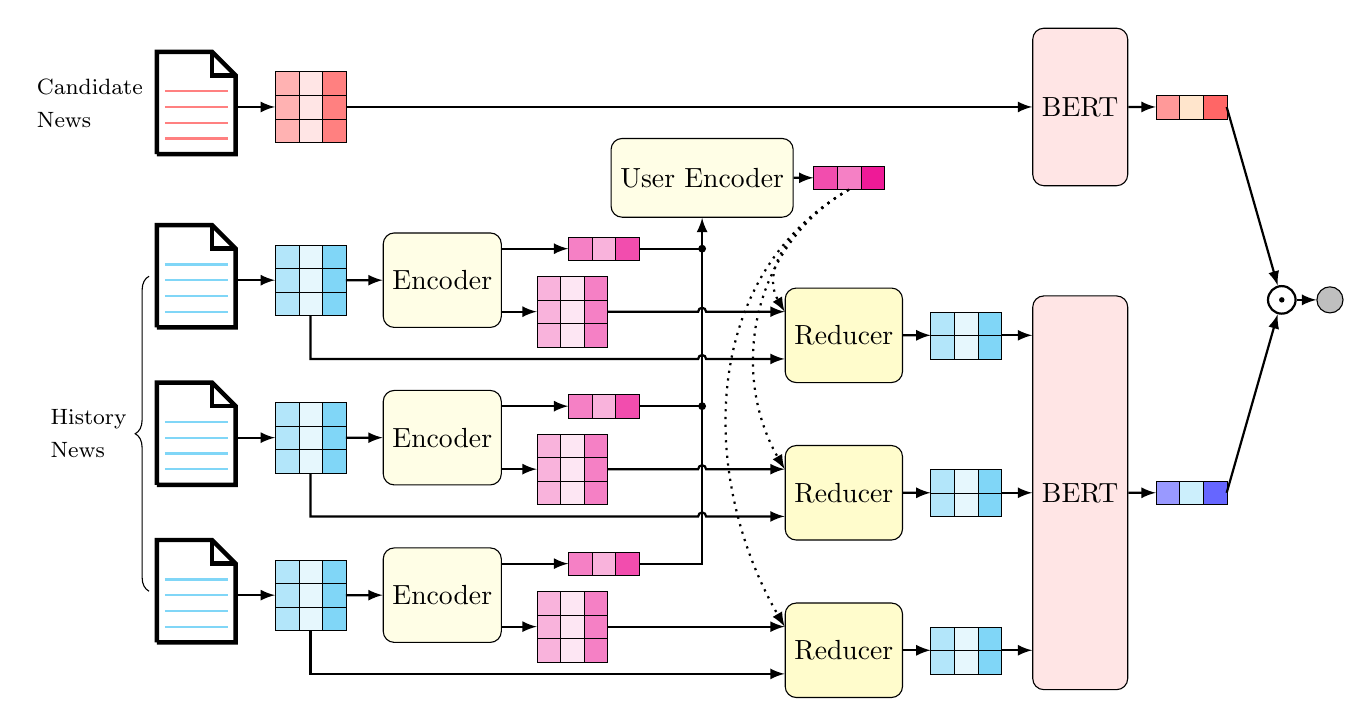
\begin{tikzpicture}[>=latex]
        \coordinate(embedding2encoderN) at (-1.2,0.4);
        \coordinate(embedding2news) at (-1.5,-0.15);
        \coordinate(embedding2repr) at (0.4,0.8);
        \coordinate(embedding2reducer) at (3,-0.3);
        \coordinate(reducer2embedding) at (0.8,0);

        \coordinate(repr2encoderU) at (0.8,0.9);
        \coordinate(encoderU2user) at (0.7,0);
        \coordinate(embedding2corner) at (0.5,0);
        \coordinate(hs2bert) at (1, 0);
        \coordinate(c2bert) at (0.2, 0);
        \coordinate(bert2cls) at (0.8, 0);
        \coordinate(cls2score) at (0.7, 0);

        \coordinate(cddemb2hisemb) at (0,-2.2);
        \coordinate(hisemb2hisemb) at (0,-2);


        % \embedding[magenta]{c}{(0,5)}
        \coordinate(c) at (0,5);
        \embedding[magenta]{h1}{($(c) + (cddemb2hisemb)$)}
        \embedding[magenta]{h2}{($(h1) + (hisemb2hisemb)$)}
        \embedding[magenta]{h3}{($(h2) + (hisemb2hisemb)$)}


        % \begin{scope}[local bounding box=repr1]
        %     \coordinate(anchor) at ($(c) + (embedding2repr) + (-0.15,-0.15)$);
        %     \draw[draw=black, dashed, ultra thin, fill=magenta!30] (anchor) rectangle ++(0.3,0.3);
        %     \draw[draw=black, dashed,ultra thin, fill=magenta!50] ($(-0.3,0) + (anchor)$) rectangle ++(0.3,0.3);
        %     \draw[draw=black, dashed, ultra thin, fill=magenta!70] ($(0.3,0) + (anchor)$) rectangle ++(0.3,0.3);
        % \end{scope}
        \vectorDark[magenta]{repr2}{($(h1) + (embedding2repr)$)}
        \vectorDark[magenta]{repr3}{($(h2) + (embedding2repr)$)}
        \vectorDark[magenta]{repr4}{($(h3) + (embedding2repr)$)}

        \node[] (enc1) at ($(embedding2encoderN) + (c.west)$) {};
        \node[encoderN] (enc2) at ($(embedding2encoderN) + (h1.west)$) {Encoder};
        \node[encoderN] (enc3) at ($(embedding2encoderN) + (h2.west)$) {Encoder};
        \node[encoderN] (enc4) at ($(embedding2encoderN) + (h3.west)$) {Encoder};

        \embedding[red]{ec}{($(enc1.west) + (-2,0)$)}
        \embedding{eh1}{($(ec) + (cddemb2hisemb)$)}
        \embedding{eh2}{($(eh1) + (hisemb2hisemb)$)}
        \embedding{eh3}{($(eh2) + (hisemb2hisemb)$)}

        \news[red]{cn}{($(ec.south west) + (embedding2news)$)}
        \news{hn1}{($(eh1.south west) + (embedding2news)$)}
        \news{hn2}{($(eh2.south west) + (embedding2news)$)}
        \news{hn3}{($(eh3.south west) + (embedding2news)$)}

        \node[encoderU] (encu) at ($(repr2encoderU) + (repr2.east)$) {User Encoder};
        \node[reducer] (red1) at ($(h1.east) + (embedding2reducer)$) {Reducer};
        \node[reducer] (red2) at ($(h2.east) + (embedding2reducer)$) {Reducer};
        \node[reducer] (red3) at ($(h3.east) + (embedding2reducer)$) {Reducer};


        \vectorDarkDark[magenta]{user}{($(encoderU2user) + (encu.east)$)}

        \embeddingS{hs1}{($(red1.east) + (reducer2embedding)$)}
        \embeddingS{hs2}{($(red2.east) + (reducer2embedding)$)}
        \embeddingS{hs3}{($(red3.east) + (reducer2embedding)$)}

        \node[bert] (berth) at ($(hs2.east) + (hs2bert)$) {BERT};
        \node[bert, minimum height=2cm] (bertc) at (berth.north |- ec.west) {BERT};
        \begin{scope}[local bounding box=hcls]
            \coordinate(anchor) at ($(berth.east) + (bert2cls) + (-0.15,-0.15)$);
            \draw[draw=black, ultra thin, fill=cyan!20] ($(anchor)$) rectangle ++(0.3,0.3);
            \draw[draw=black, ultra thin, fill=blue!40] ($(-0.3,0) + (anchor)$) rectangle ++(0.3,0.3);
            \draw[draw=black, ultra thin, fill=blue!60] ($(0.3,0) + (anchor)$) rectangle ++(0.3,0.3);
        \end{scope}

        \begin{scope}[local bounding box=ccls]
            \coordinate(anchor) at ($(bertc.east) + (bert2cls) + (-0.15,-0.15)$);
            \draw[draw=black, ultra thin, fill=orange!20] ($(anchor)$) rectangle ++(0.3,0.3);
            \draw[draw=black, ultra thin, fill=red!40] ($(-0.3,0) + (anchor)$) rectangle ++(0.3,0.3);
            \draw[draw=black, ultra thin, fill=red!60] ($(0.3,0) + (anchor)$) rectangle ++(0.3,0.3);
        \end{scope}

        \node[circle, minimum size=0.35cm, thick, draw=black] (dot) at ($0.5*(ccls.east) + 0.5*(hcls.east) + (cls2score)$) {};
        \node[circle,fill,inner sep=0.7pt] at (dot.center) {};
        \node[circle, draw=black, fill=gray!50, thin, radius=0.5] (score) [right=0.25 of dot] {};

        \draw[line] (cn.east |- ec.west) -- (ec.west);
        \draw[line] (hn1.east |- eh1.west) -- (eh1.west);
        \draw[line] (hn2.east |- eh2.west) -- (eh2.west);
        \draw[line] (hn3.east |- eh3.west) -- (eh3.west);
        \draw[line] (ec.east) -- (bertc.west);
        \draw[line] (eh1.east) -- (enc2.west);
        \draw[line] (eh2.east) -- (enc3.west);
        \draw[line] (eh3.east) -- (enc4.west);
        \draw[line] (enc2.east |- h1.west) -- (h1.west);
        \draw[line] (enc3.east |- h2.west) -- (h2.west);
        \draw[line] (enc4.east |- h3.west) -- (h3.west);
        \draw[line] (enc2.east |- repr2.west) -- (repr2.west);
        \draw[line] (enc3.east |- repr3.west) -- (repr3.west);
        \draw[line] (enc4.east |- repr4.west) -- (repr4.west);

        \coordinate(corner) at ($(encu.south)$);
        \draw[line] (repr4.east) -| (corner);
        \draw[thick] (repr3.east) -- (repr3.east -| corner);
        \draw[thick] (repr2.east) -- (repr2.east -| corner);

        \draw[line] (encu.east) -- (user.west);
        % add connection dot
        \node[circle,fill,inner sep=1pt] at (repr3.east -| corner) {};
        \node[circle,fill,inner sep=1pt] at (repr2.east -| corner) {};

        \draw[line,dotted] (user.south) to [out=-150,in=120] (red1.west |- h1.east);
        \draw[line,dotted] (user.south) to [out=-150,in=120] (red2.west |- h2.east);
        \draw[line,dotted] (user.south) to [out=-150,in=120] (red3.west |- h3.east);

        \draw[line] (h1.east) -- ($(h1 -| corner) + (-0.05,0)$) arc (180:0:0.05) -- (red1.west |- h1.east);
        \draw[line] (h2.east) -- ($(h2 -| corner) + (-0.05,0)$) arc (180:0:0.05) -- (red2.west |- h2.east);
        \draw[line] (h3.east) -- (red3.west |- h3.east);

        \coordinate(corner2) at ($(eh2.south |- red2.west) - (red2.west |- h2.east) + (red2.west)$);
        \draw[line] (eh2.south) -- (corner2)-- ($(corner2 -| corner) + (-0.05,0)$) arc (180:0:0.05) -- ($(red2.west) - (red2.west |- h2.east) + (red2.west)$);
        \coordinate(corner2) at ($(eh1.south |- red1.west) - (red1.west |- h1.east) + (red1.west)$);
        \draw[line] (eh1.south) -- (corner2)-- ($(corner2 -| corner) + (-0.05,0)$) arc (180:0:0.05) -- ($(red1.west) - (red1.west |- h1.east) + (red1.west)$);
        \coordinate(corner2) at ($(eh3.south |- red3.west) - (red3.west |- h3.east) + (red3.west)$);
        \draw[line] (eh3.south) -- (corner2) -- ($(red3.west) - (red3.west |- h3.east) + (red3.west)$);

        \draw[line] (red1.east) -- (hs1.west);
        \draw[line] (red2.east) -- (hs2.west);
        \draw[line] (red3.east) -- (hs3.west);

        \draw[line] (hs1.east) -- (berth.west |- hs1.east);
        \draw[line] (hs2.east) -- (berth.west |- hs2.east);
        \draw[line] (hs3.east) -- (berth.west |- hs3.east);

        \draw[line] (berth.east) -- (hcls.west);
        \draw[line] (bertc.east) -- (ccls.west);

        \draw[line] (ccls.east) -- (dot);
        \draw[line] (hcls.east) -- (dot);
        \draw[line] (dot) -- (score);

        \draw[decorate,decoration={brace,amplitude=5pt,mirror}]($(hn1.west) + (-0.1,0)$) -- ($(hn3.west) + (-0.1,0)$);
        \node[text width=1.3cm] [left=0.1 of cn] {\footnotesize Candidate News};
        \node[text width=1.3cm] at ($0.5*(hn3.west) + 0.5*(hn1.west) + (-0.7,0)$) {\footnotesize History News};

    \end{tikzpicture}
\end{document}